\documentclass[a4paper]{article}

\usepackage{authblk}
\usepackage{kotex, amsmath,amssymb,amsthm, mathtools, physics}
\usepackage{tikz,titlesec,hyperref, enumitem, systeme, bbm}
\usepackage{csquotes}
\usepackage[ruled,vlined]{algorithm2e}
\usepackage{optidef}
\usepackage{arydshln}
\usepackage{xcolor}
\usepackage{subfig}
\usepackage[normalem]{ulem}

\newtheorem{theorem}{Theorem}[section]
\newtheorem{corollary}{Corollary}[theorem]
\newtheorem{lemma}[theorem]{Lemma}

\newtheorem*{remark}{Remark}

\usepackage[a4paper,margin=2cm]{geometry}

\linespread{1.3}

\newtheorem{claim}{Claim}[section]


\newcommand\name{Junghyun Lee}   % Name of the student
\newcommand\university{KAIST} % Name of the university
\newcommand\department{Dept. of Mathematical Sciences \& School of Computing} % Name of the department
\newcommand\studentid{20170500} % Student ID

\title{(CS454) Report for:\\
	{\it Solving TSP using Stochastic Optimization} \bigskip}
\author{\textbf{\Large \name}\thanks{jh\_lee00@kaist.ac.kr} \ (\studentid) \\
\department, \university}
\date{\today}

\begin{document}
\thispagestyle{empty}
\maketitle
\tableofcontents
\newpage


\begin{figure}[htp] 
	\centering
	\subfloat[A motivating example from the GTSRB dataset]{%
		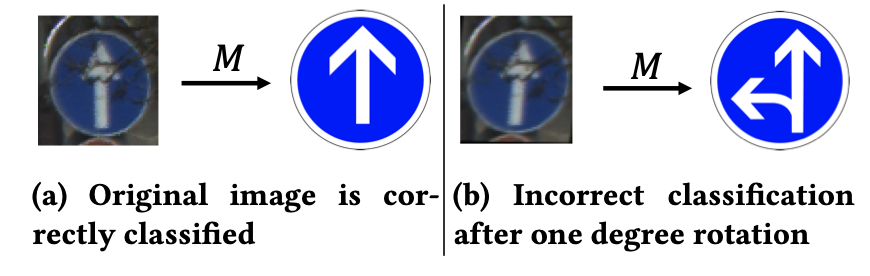
\includegraphics[width=0.46\textwidth]{fig1.png}%
		\label{fig:1a}%
	}%
	\hfill%
	\subfloat[An overview of \textsc{Sensei} for one seed image in one epoch.]{%
		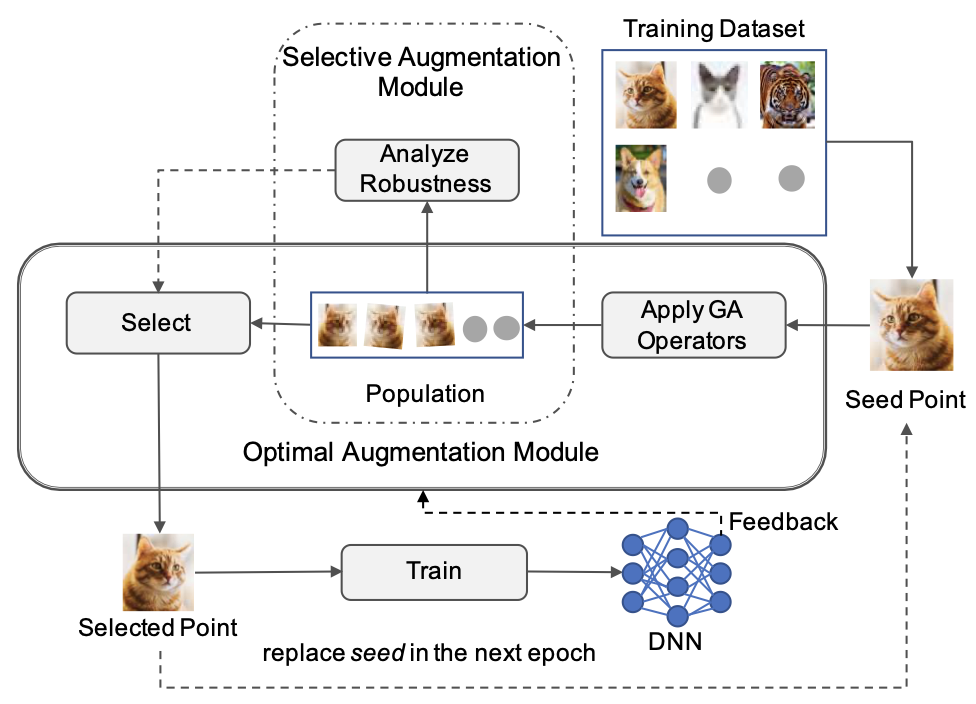
\includegraphics[width=0.46\textwidth]{fig3.png}%
		\label{fig:1b}%
	}%
	\caption{Figures from \cite{GSPR20}}
	\label{fig:1}
\end{figure}


\section{Background}


\section{Algorithm}



\newpage
\bibliographystyle{ieeetr}
\bibliography{bibliography}{}
%\nocite{*}

\end{document}
